\documentclass[a4paper]{article}
\usepackage{amsmath,graphicx,geometry,booktabs,epstopdf,float,wrapfig,setspace,colortbl,color,subfigure,palatino,ulem,listings,fontspec,hyperref,url}
\usepackage[table,xcdraw]{xcolor}
\usepackage[T1]{fontenc}
\setmainfont{CMU Serif Roman}
\geometry{a4paper,left=2.54cm,right=2.54cm,top=2.54cm,bottom=2.54cm}
\linespread{1.3}
\newfontfamily\menlo{Menlo}
\renewcommand\thesection{\Roman{section}}
\renewcommand\thesubsection{\indent{\Alph{subsection}}}
\begin{document}
\title{\textbf{Project 1 Report}}
\author{Gu Yucheng}
\maketitle
\begin{table}[ht]
\centering
\begin{tabular}{ll}
\multicolumn{2}{c}{\textbf{Data Structures and Algorithms}}        \\
\multicolumn{2}{c}{\textbf{VE281}}                                 \\
\multicolumn{2}{l}{}                                               \\
Student ID     & 518370910168                                      \\
E-mail Address & \textit{enoch2090@sjtu.edu.cn}
\end{tabular}
\end{table}

\begin{table}[b]
\centering
\begin{tabular}{c}
University of Michigan-Shanghai Jiao Tong University Joint Institute(UM-SJTU JI)\\
\end{tabular}
\end{table}

\thispagestyle{empty}
\newpage
\setcounter{page}{1}
\section{Runtime of different Sorting Algorithms}
    \par{} The 6 sorting algorithms are tested along with std::sort\(\), and the results are shown as table 1. Note for the following points:
    \begin{enumerate}
        \item For each run, a random input vector of selected length is generated and tested upon the 7 algorithms.
        \item For input length less than 10,000, the listed time in the table is the average time over 5 different runs. For other inputs, the listed time is the time of one run over a random input vector.
        \item For the inplace quicksort, my algorithm on JOJ has a typo at line 182, which writes "int front = left;" while the correct version is "int front = left + 1;". This will cause the pivot be swapped inside the array, and though the results are usually correct, the runtime is roughly $O\left(n^2\right)$. The data listed in the table uses the corrected version of algorithm.
    \end{enumerate}
    The following data is tested on Ubuntu 18.04 VM inside macOS Mojave 10.14, with:
    \begin{equation*}
        \begin{aligned}
        &\mathrm{CPU:\;2.9\,GHz\;Intel\;Core\;i9}\\
        &\mathrm{Memory:\;16\,GB\;2400\,MHz\;DDR4}
        \end{aligned}
    \end{equation*}
    And all time data is retrieved via C++11 chrono library.
    \begin{table}[H]
        \centering{}
        \begin{tabular}{|c|c|c|c|c|c|c|c|}
        \hline
        \rowcolor[HTML]{EFEFEF} 
        Input  & Bubble    & Selection & Insertion & Merge      & QSort Extra & QSort Inplace & std::sort \\ \hline
        10     & 0.000001  & 0.0000006 & 0.0000002 & 0.00000275 & 0.0000072   & 0.0000052     & \multicolumn{1}{l|}{0.000001}               \\ \hline
        50     & 0.0000196 & 0.000012  & 0.0000082 & 0.0000178  & 0.0000468   & 0.0000372     & 0.0000076                                   \\ \hline
        1000   & 0.006826  & 0.00311   & 0.0020886 & 0.0004646  & 0.0009928   & 0.000769      & 0.0002254                                   \\ \hline
        5000   & 0.14976   & 0.0662254 & 0.0447926 & 0.0043702  & 0.0045666   & 0.003372      & 0.0011384                                   \\ \hline
        10000  & 0.750991  & 0.332596  & 0.205324  & 0.016368   & 0.012091    & 0.009207      & 0.003187                                    \\ \hline
        50000  & 17.638818 & 7.724575  & 5.44553   & 0.364424   & 0.056839    & 0.046142      & 0.018546                                    \\ \hline
        100000 & 71.274057 & 31.117099 & 20.566528 & 1.641047   & 0.132166    & 0.098491      & 0.038946                                    \\ \hline
        \end{tabular}
        \caption{Runtime of different algorithms over different size of input}
    \end{table}
    Plotting the runtime versus input size yields:
    \begin{figure}[H]
        \centering{}
        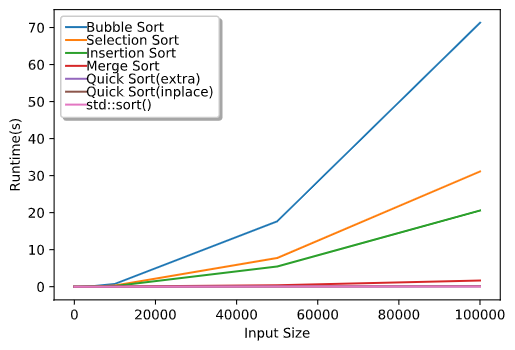
\includegraphics[width = .65\textwidth]{Figures/fig1.png}
        \centering
        \caption{Runtime of different algorithms versus input size}
    \end{figure}
    Taking logarithm of both axis:
    \begin{figure}[H]
        \centering{}
        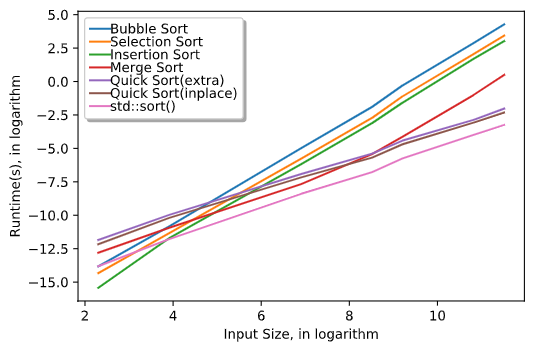
\includegraphics[width = .65\textwidth]{Figures/fig2.png}
        \centering
        \caption{Runtime of different algorithms versus input size, both axis taken logarithm}
    \end{figure}
\section{Analysis of the result}
    \par{} From the result, we can readoff the following conclusions:
    \begin{enumerate}
        \item For small number of input$\left( <50 \right)$, bubble sort, selection sort and insertion sort is faster. This is because the constant factor of the
        \item For large number of input$\left( \geq 1000 \right)$, merge sort and quick sort is faster. This is because they are in $O\left(nlogn\right)$ time, which is faster than $O\left(n^2\right)$ time of the first three algorithms as n grows large.
        \item For std::sort, when input size is small it's close to the speed of bubble sort, selection sort and insertion sort; while when input size is large it's close to the speed of merge sort and quick sort. According to the internet, the implementation of std::sort\(\) uses a method called "Introspective Sorting". The original artical published by David Musser can be found at \url{http://citeseerx.ist.psu.edu/viewdoc/summary?doi=10.1.1.14.5196}. When the input is large, the algorithm uses sorting algorithm of $O\left(nlogn\right)$. When the segment to sort in some recursion is smaller than a threshold, it changes to insertion sort to achieve nearly $O\left(n\right)$ speed because the segment is probably already ordered. When the recursion level is too deep, it turns to heap sort which is also $O\left(nlogn\right)$, but has a large constant. In all, this algorithm balances the trade-offs of time and space.
    \end{enumerate}
\section*{Reference}
    \begin{enumerate}
        \item David Musser, Introspective Sorting and Selection Algorithms, \url{http://citeseerx.ist.psu.edu/viewdoc/summary?doi=10.1.1.14.5196}
    \end{enumerate}
\end{document}
